\documentclass{article}
%\usepackage{nicematrix}
\usepackage{amssymb,amsmath,amsthm}
\usepackage{amsfonts,mathtools}
\usepackage{stackengine}
\stackMath
%\usepackage{graphicx}
%\usepackage{nicematrix}
%\usepackage{blkarray}
\usepackage{tikz}
\usepackage{tkz-euclide,subfigure} 
\usepackage{amsthm}
\newtheorem{theorem}{Theorem}[section]
\newtheorem{acknowledgement}[theorem]{Acknowledgement}
%\newtheorem{conjecture}[theorem]{Conjecture}
\newtheorem{corollary}[theorem] {Corollary}
\newtheorem{definition}[theorem]{Definition}
\newtheorem{example}[theorem]{Example}
\newtheorem{lemma} [theorem]{Lemma}
%\newtheorem{notation}[theorem]{Notation}
%\newtheorem{observation}[theorem]{Observation}
%\newtheorem{problem}[theorem]{Problem}
\newtheorem{proposition}[theorem]{Proposition}
\newtheorem{remark}{Remark}[section]

\newtheorem{problem}[theorem]{Problem}
\newtheorem*{open problem*}{Open Problem}

\newtheorem{conjecture}{Conjecture}
%\usepackage{caption}
%\usepackage{tikz}
%\usepackage{kbordermatrix}


%\renewcommand{\kbldelim}{(}% Left delimiter
%\renewcommand{\kbrdelim}{)}% Right delimiter
\voffset=-12mm
\mathsurround=2pt
\parindent=12pt
\parskip= 4.5 pt
\lineskip=3pt
\oddsidemargin=10mm
\evensidemargin=10mm
\topmargin=55pt
\headheight=12pt
\footskip=30pt
\textheight 8.1in
\textwidth=150mm
\raggedbottom
\pagestyle{myheadings}
\hbadness = 10000
\tolerance = 10000
\let\espffile=\espfbox


\renewcommand{\refname}{
	\begin{center}
		\normalsize \bf References
	\end{center}
}
\vspace{5cm}

\begin{document}
	
	\label{'ubf'}  
	\setcounter{page}{1}                                 %Put here the starting page number
	
	
	\markboth {\hspace*{-9mm} \centerline{\footnotesize \sc
			% Put here the left page top label 
			Dual of splitting $p$-matroids}
	}
	{ \centerline                           {\footnotesize \sc  
			%put here the author's name
			Amol Narke$^1,$ Prashant Malavadkar $^2,$ Maruti M. Shikare$^3$                                               } \hspace*{-9mm}              
	}
	
	
	\begin{center}
		{ 
			{\Large \textbf { \sc Bounds on Path Energy of Graphs
				}
			}
			\\
			
			
			\medskip
			
			
			
			
			{\sc Amol Narkel$^1,$ Prashant Malavadkar$^2,$ Maruti M. Shikare$^3$}\\
			{\footnotesize  Department of Mathematics and Statistics, Dr. Vishwanath Karad MIT-World Peace University, Pune-38, India. }\\
			{\footnotesize e-mail: {\it 1. amol.narke@mitwpu.edu.in 2. prashant.malavadkar@mitwpu.edu.in 3.mmshikare@gmail.com }}
		}
	\end{center}
	
	
	\thispagestyle{empty}
	
	
	\hrulefill
	
	
	\begin{abstract}  
		{\footnotesize 
			Given a graph $M,$ path eigenvalues are eigenvalues of its path matrix. The path energy of a simple graph $M$ is equal to the sum of the absolute values of the path eigenvalues of the graph $M$ (Shikare et. al, 2018). We have discovered new upper constraints on path energy in this study, expressed in terms of a graph's maximum degree. Additionally, a relationship between a graph's energy and path energy is given.}
		\end{abstract}
		\hrulefill
		
		\section{Introduction}
	The energy of a graph was introduce in 1978 by I. Gutman \cite{ge1}. If $M$ be a simple graph then $P(M)$ be its path matrix defined by Patekar and Shikare in 2016 as follows,
	\begin{definition}\cite{pe1}
		Let $M$ be a simple graph, and let $V (M)=v_1, v_2, \ldots, v_k.$ be its vertex set. Define the path matrix of graph $M$ as matrix $P = (p_{ij})$ of dimension $k \times k$, where $p_{ij} = 0$ if $i = j$ and equals the maximum number of vertex disjoint paths from $v_i$ to $v_j$ if $i \neq j.$
	\end{definition}
	The spectrum of path matrix is denoted by $Spec_P(M)$.
	Consider the following example,
	\begin{figure}[ht]\label{example1}\centering
		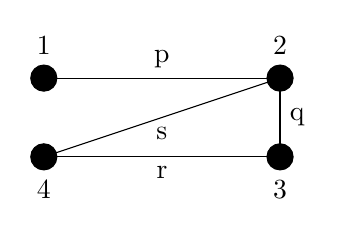
\begin{tikzpicture}
			\node [shape= circle, draw, label=below:4, fill=black] (4) at (-3, 0) {};
			\node [shape= circle, draw, label=below:3, fill=black] (3) at (0, 0) {};
			\node [shape= circle, draw, label=2, fill=black] (2) at (0, 1) {};
			\node [shape= circle, draw, label=1, fill=black] (1) at (-3, 1) {};
			\draw (1.center) to node[above] {p} (2.center);
			\draw (2.center) to node[right] {q}(3.center);
			\draw (3.center) to node[below] {r} (4.center);
			%\draw (4.center) to node[left] {a} (1.center);
			\draw (4.center) to node[below] {s} (2.center);
		\end{tikzpicture}
		\caption{\bf{M}}
	\end{figure}
	
	The path matrix for a graph $M$ is,
	\begin{equation*}
		P(M) =
		\begin{bmatrix}
			0 & 1 & 1 & 1 \\
			1 & 0 & 2 & 2 \\
			1 & 2 & 0 & 2 \\
			1 & 2 & 2 & 0 \\
		\end{bmatrix}
	\end{equation*}
	$Spec_P(M)=\{-2, -2, 4.6457, -0.6457\}.$
	\begin{definition}\cite{cn}
		The path energy of graph $M$ is represented by $PE = PE(M)$, which is equal to sum of  absolute values of the path eigenvalues. 
	\end{definition}	
	The path energy $PE(M)$ of the graph $M$ shown in Figure $1$ is, $\mid-2\mid+\mid-2\mid+\mid4.6457\mid+\mid-0.6457\mid=9.2914.$
	
	The path eigenvalues of the $r$-regular graph $M$ on $k$ vertices are $–r$ with multiplicity $k-1$ and $r(k-1)$ with multiplicity $1$, according to the authors' findings in  \cite{cn}. When this fact is applied to a $r$-regular graphs, the following outcomes occur.  
	\begin{theorem}\label{pek}
		Path energy of a $r$-regular graph on $k$ vertices is $2r(k-1).$     
	\end{theorem}
	Using Theorem \ref{pek} and the fact that $L(K_p)$ is  $2(p-2)$-regular on $p(p-1)/2$ vertices and $L(K_{p,q})$ is $(p+q-2)$-regular on $pq$ vertices respectively. We get following corollaries.  
	\begin{corollary}\label{pel}
		Path energy of $L(K_p)$ is $2(p+1)(p-2)^2$.
	\end{corollary}
	\begin{proof}
		$K_p$ is a complete graph on $p$ vertices with $p(p-1)/2$ edges. Each edge of $K_p$ is adjacent to $2(n-2)$ distinct edges. Thus, in a line graph of $K_p$ each vertex has degree $2(p-2)$, so $L(K_p)$ is $2(p-2)$-regular on $p(p-1)/2$ vertices. Using the theorem \ref{pek} we conclude the proof.
	\end{proof}
	\begin{corollary}
		Path energy of $L(K_{p,q})$ is $2(p+q-2)(pq-1),$ for $p \geq 1$ and $q \geq 1.$
	\end{corollary}
	Proof follows from Theorem \ref{pek} stated above and Theorem 2.2 from \cite{kbg}.
	\begin{corollary}
		Prism graph $Y_p$ also called as circular ladder graph on $2p$ vertices, have path energy $6(2p-1)$ and antiprism graph $Y^{'}_{p}$ have path energy $8(2p-1)$, Moreover $PE(Y_p)=\dfrac{3}{4} PE(Y^{'}_{p})$
	\end{corollary}
	\begin{proof}
		Prism graph $Y_p$ has $2p$ vertices and $3p$ edges and it is $3$-regular graph. $Y^{'}_{p}$ is $4-$regular, consisting of $2p$ vertices and $4p$ edges. Using the theorem \ref{pek} we get $PE(Y_p)=6(2p-1)$ and $PE(Y^{'}_{p})=8(2p-1).$
	\end{proof}
	
	In 2016, Patekar and Shikare \cite{pe1} have found path eigenvalues of some graphs. In Table \ref{tab:Table 1} we have observed that all graphs in Table \ref{tab:Table 1} has only one positive eigenvalue which is path spectral radius ($\rho$) of that graph. Thus for such graphs we can easily obtained path energy which is equal to $PE(M)=2\rho$
	\begin{proposition}
		Let $M$ be a simple connected graph with only one positive path eigenvalue then this path eigenvalue is path spectral radius of $M$ called $\rho.$ Moreover $PE(M)=2\rho.$  
	\end{proposition}     
	\begin{proof}
		Let $P(M)$ be a path matrix of simple connected graph $M$ on $p$ vertices with path eigenvalues $\beta_1,\beta_2, \ldots, \beta_n.$ Without loss of generality assume that $\beta_1 > 0$ and for $i\geq2,$ $\beta_i < 0.$ As trace of the path matrix is always zero this implies that $\beta_1+ \beta_2+\beta_3 +\ldots+\beta_n=0$ gives us, $\beta_1= -\beta_2-\beta_3 -\ldots-\beta_n.$ On the contrary assume that $\beta_1$ is not a path spectral radius of $M$ then for some integer $k$ such that $2 \leq k\leq p,$ $|\beta_k|$ be a path spectral radius of $M$ that is $|\beta_k|>|\beta_1|$. Consider, $\beta_1= -\beta_2-\beta_3 -\ldots-\beta_n$ implies that $|\beta_1|= |\beta_2|+|\beta_3| +\ldots+|\beta_n|.$ This contradict the fact that $|\beta_k|>|\beta_1|$. Thus $\beta_1$ is path spectral radius of $M.$ Moreover, $PE(M)=|\beta_1|+ |\beta_2|+|\beta_3| +\ldots+|\beta_n|$ as $\beta_1= \beta_2+\beta_3 +\ldots+\beta_n.$ Gives us $PE(M)=2\beta_1=2\rho.$      
	\end{proof}
	\begin{center}
		Following is the list of some graphs having only one positive path eigenvalue ($\rho$) and path energy $2\rho$. 
		\begin{table}[ht]
			\renewcommand{\arraystretch}{1}
			\begin{tabular}{|c | c |} 
				\hline
				Graphs & Path eigenvalues \\ 
				\hline
				$K_p$ & $ \begin{pmatrix}
					(p-1)^2 & (-p+1) \\
					1 & (p-1) \\
				\end{pmatrix}$ \\ 
				\hline
				($r$-regular graph)$_p$ & $\begin{pmatrix}
					r(p-1) & (-r) \\
					1 & (p-1) \\
				\end{pmatrix}$ \\
				\hline
				$T_p$ &$\begin{pmatrix}
					(p-1) & (-1) \\
					1 & (p-1) \\
				\end{pmatrix}$ \\
				\hline
				$K_{p,q}$ & $\begin{pmatrix}
					\frac{p(q-1)+ q(p-1)\pm\sqrt{(p-q)^2+4p^3q}}{2} & (-q) & (-p)\\
					1 & (p-1) & (q-1)\\
				\end{pmatrix}$ \\
				\hline
				$\mathcal{Q}_{p}$ & $\begin{pmatrix}
					p(2^p-1) & (-1) \\
					1 & (2^p-1) \\
				\end{pmatrix}$ \\  
				\hline
				$\mathcal{Q}_{p}\times \mathcal{Q}_{q}$ & $\begin{pmatrix}
					(q+p)(2^{q+p}-1) & -(q+p) \\
					1 & 2^{q+p}-1 \\
				\end{pmatrix}$ \\
				\hline
				$W_p$ & $\begin{pmatrix}
					3(p-1) & -3 \\
					1 & (p-1) \\
				\end{pmatrix}$ \\
				\hline
			\end{tabular}
			\caption{\label{tab:Table 1}Graphs having only one positive path eigenvalue}
		\end{table}
	\end{center}        
	\begin{conjecture}\label{conjecture1}
		If $M$ is $2$-connected graph then its path matrix has exactly one positive eigenvalue.  
	\end{conjecture}
	Note that: The converse of the above Conjecture \ref{conjecture1} is not true that is, If path matrix has exactly one positive eigenvalue then its corresponding graph may not be $2$-connected.  
	\begin{example}
		The eigenvalues of any tree on $p$ vertices have path spectrum $\{(p-1),-1, -1,$\ldots$,-1_{(p-1) \text{times}}.\}$
	\end{example}
	\begin{example}
		In \cite{Aleksandar Ilic}, Ilic proved that path matrix of unicyclic graph on $p$ verices has two positive path eigenvalues if $p\geq 7$ and $3\leq p \leq (p-3)$. 
	\end{example}
	
	\begin{conjecture}\label{Conjecture2}
		If the graph $M$ can be decomposed in to $k$  $2$-connected components then path matrix of $M$ has exactly $k$ positive eigenvalues.
	\end{conjecture}
	\section {New bounds for path energy}
	In the following proposition we have found upper bound for row sum of path matrix in term of degree of vertices.  
	\begin{proposition}\label{bounds}
		$M$ be a graph on $p$ vertices then,
		$$\sum_{i\neq j=1}^{p} p_{i,j} \leq (p-1)d(v_i),$$ for $i\neq j=1,2,\dots,p.$
	\end{proposition}
	
	\begin{proof}
		We fixed $i$, $p_{i,j}$ is at most degree of $v_i$ for all $i \neq j=1,\dots,p$ and for $i=j$ it is $0.$ That is,\\
		$$ p_{i,j} \leq d(v_i)$$
		taking summation over $j$, we get $$ \sum_{j \neq i=1}^{p} p_{i,j} \leq \sum_{j \neq i=1}^{p} d(v_i).$$ 
	\end{proof}
	Following theorem gives the upper bound for absolute eigenvalue of path matrix in terms of maximum vertex degree of a graph.     
	\begin{theorem} \label{mev}
		Let $M$ be a graph on $p$ vertices, with path matrix $P(M)$. $\Delta$ be the maximum degree of $M.$ If $\beta$ is an eigenvalue of $P(M)$ then $|\beta|\leq (p-1)\Delta$.  
	\end{theorem}
	\begin{proof}
		Let $x$ be an eigenvector of $P(M)$ corresponding to eigenvalue $\beta,$ then $Px=\beta x.$
		Write $x=(x_1, x_2,x_3,...,x_p)^t$ where without loss of generality, $|x_1|=\underset{ 1\leq i \leq p}\max|x_i|.$ 
		$|\beta||x_1|=\displaystyle\sum_{j \neq i=1}^{p} p_{1,j} x_j 
		\leq |x_1|\sum_{j \neq i=1}^{p} p_{1,j}$
		$\leq |x_1| (p-1) deg(v_i)	
		\leq |x_1| (p-1) \Delta
		\leq |x_1| (p-1) \Delta.$ 
	\end{proof}
	Aleksandar Ilic et al. \cite{Aleksandar Ilic}  proved the conjecture $PE(M)\leq 2(p-1)^2$ stated in Shikare et. al \cite{pe1}. In the following corollary we obtained a bound for path energy of graph in term of total number of edges.
	\begin{corollary}
		Let $M$ be graph on $p$ vertices and $m$ edges. Then $PE(G) \leq 2(p-1)m.$
	\end{corollary}
	
	\begin{proof}
		Theorem \ref{mev} gives us  
		\begin{equation}
			|\beta|\leq (p-1)deg(v_i)	 
		\end{equation}
		This is true for every $|\beta|,$ taking summation over $i$ we get,
		\begin{equation}
			\sum_{i=1}^{p} |\beta|\leq (p-1) \sum_{i=1}^{p} deg(v_i) \leq (p-1)(2m).
		\end{equation}
		Thus we get $PE(M) \leq 2(p-1)m.$ 
	\end{proof}
	
	\begin{corollary} \label{enq}	
		Let $M$ be a graph on $p$ vertices. $\Delta$ be the maximum vertex degree of $M$ then $PE(M) \leq p(p-1) \Delta.$
	\end{corollary}
	\begin{proof}
		We have $|\beta|\leq (p-1) \Delta$ for every $|\beta|.$ Taking summation over $\beta \in Spec_P,$ we get $PE(M) \leq p(p-1) \Delta.$    
	\end{proof}
	A relation between energy of graph and path energy of graph is given in the following corollary. 
	\begin{corollary}
		Let $M$ be a connected graph on $p$ vertices and $\Delta$ be the maximum vertex degree of a graph $M$ then $ E(M) \leq \dfrac{p}{2} PE(M) \leq \dfrac{p^2(p-1)\Delta}{2}$. Equality holds if $M=K_2.$  
	\end{corollary}
	
	\begin{proof}
		Let $M$ be a connected graph on $p$ vertices. Ilic et al. \cite{Aleksandar Ilic} proved the inequality $2(p-1) \leq PE(M).$ By using Corollary \ref{enq}, $PE(M) \leq p(p-1) \Delta.$ Thus,
		\begin{equation}\label{pe_in_1}
			(p-1) \leq \dfrac{PE(M)}{2} \leq \dfrac{p(p-1)\Delta}{2}.
		\end{equation}
		Let $A(M)$ be an adjacency matrix of $M.$
		And $x$ be an eigenvector of $A(M)$ corresponding to eigenvalue $\beta'$ then,
		\begin{center}
			$Ax'=\beta' x'$
		\end{center}
		Write $x'=(x_1', x_2',x_3',...,x_p')^t$ where without loss of generality, $|x_1'|=\underset{ 1\leq i \leq p}\max|x_i'|.$ Now, 
		\begin{equation}
			|\beta'||x_i'|=\sum_{j=1}^{p} a_{1j}x_j' 
			\leq |x_1'|\sum_{j=1}^{p} a_{1j}
			\leq |x_1'| deg(v_i)	
			\leq |x_1'|  \Delta(v)
			\leq |x_1'| \Delta(v). 
		\end{equation} \\
		Taking summation over $\beta' \in Spec_M$ we get,	$E(M)\leq p\Delta.$ As $M$ is simple connected graph, $\Delta = (p-1).$ Thus,
		\begin{equation}\label{ee_in_1}
			E(G)\leq p(p-1).
		\end{equation}
		Combining equations \ref{pe_in_1} and \ref{ee_in_1} we get, $E(M) \leq \dfrac{p}{2} PE(M) \leq \dfrac{p^2(p-1)\Delta}{2}.$ 
		Further the equality holds if $M$ is $K_2.$
	\end{proof}

	
	\begin{thebibliography}{00}
		
		\bibitem{akbari path energy} S. Akbari, A. H. Ghodrati, I. Gutman, M. A. Hosseinzadeh, E. V. Konstantinova, On path energy of graphs, \textit{MATCH Commun. Math. Comput. Chem.\/} \textbf{81} (2019) 465–470.
		
		\bibitem{akbari bicyclic graph}  S. Akbari, A. H. Ghodrati, M. A. Hosseinzadeh, S. S. Akhtar, On the path energy of bicyclic graphs, \textit{MATCH Commun. Math. Comput. Chem.\/} \textbf{81} (2019) 471–484.
		
		\bibitem{br}R. Balakrishnan, The energy of a graph, \textit{Linear Algebra Appl.}, \textbf{387} (2004) 287-295.
		
		\bibitem{eqiuenergetic trees}V. Brankov, D. Stevanovi\'c, I. Gutman, Equienergetic chemical trees, J. Serb. Chem. Soc. \textbf{69} (2004) 549-553.
		
		\bibitem{spectra of graphs} Andries E. Brouwer, Willem H. Haemers, \textit{Spectra of graphs\/}, Springer, 2011.
		
		\bibitem{ge1} I. Gutman, The energy of a graph, \textit{Ber. Math. Statist. Sekt. Forschungsz. Graz.,} \textbf{103} (1978) 1-22.
		
		\bibitem{fh} F. Harary, \textit{Graph Theory,} Addison-Wesley, Reading, MA, 1969.
		
		\bibitem{Aleksandar Ilic} Aleksandar Ilic, Milan Baši, Path matrix and path energy of graphs, \textit{Applied Mathematics and Computation,} \textbf{355} (2019) 537–541.
		
		\bibitem{pe1} S. C. Patekar, M. M. Shikare, On the path matrices of graphs and their properties, \textit{Adv. Appl. Discr. Math.,} \textbf{17},(2016) 169-184.
		
		\bibitem{cg}S. C. Patekar and Maruti M. Shikare, On the path cospectral graphs and path signless Laplacian matrix of graph, \textit{Journal of Mathematical and Computational Science.,} \textbf{10(4)} (2020) 922–935.
		
		\bibitem{equienergetic}H. S. Ramane, H. B. Walikar, S. B. Rao, B. D. Acharya, I.Gutman, P. R. Hampiholi, S. R. Jog, Equienergetic graphs, \textit{Kragujevac.J. Math.} \textbf{26} (2004) 5–13.
		
		\bibitem{cn}M. M. Shikare, P. P. Malavadkar, S. C. Patekar, I. Gutman, On path eigenvalues and path energy of graphs, \textit{MATCH Commun. Math. Comput. Chem.\/} \textbf{79} (2018) 387-398.
		
		\bibitem{kbg}KhinSandar Win, Complete Bipartite Graphs and Their Line Graphs, \textit{Dagon University Commemoration of 25th Anniversary Silver Jubilee Research Journal,} \textbf(Vol.9) (2019) No.2.
	\end{thebibliography}
	
	\end{document}
	